\documentclass[11pt]{article}
\usepackage{bookmark}
\usepackage{algorithm}
\usepackage{algpseudocode}
\usepackage{amsfonts}
\usepackage{amsmath}
\usepackage{amssymb}
\usepackage{amsthm}
\usepackage{bm}
\usepackage{color}
\usepackage{comment}
\usepackage{float}
\usepackage{graphicx}
%\usepackage[hidelinks]{hyperref}
\usepackage{makecell}
\usepackage[caption=false,font=footnotesize,subrefformat=parens,labelformat=parens]{subfig}
\usepackage{wrapfig}
\usepackage{url}
\usepackage[table]{xcolor}
\graphicspath{{images/}}
\setlength{\parindent}{0.25in}
\setlength{\parskip}{.05in}
\pagestyle{plain}
%Title, date an author of the document
\title{Progress Report}
\author{Bardia Mojra}


\begin{document}
\maketitle
\thispagestyle{empty}

\bigskip
\bigskip
\begin{center}
 Robotic Vision Lab
\end{center}

\begin{center}
The University of Texas at Arlington
\end{center}

\newpage

\section{Specific Research Goals}
\begin{itemize}
      \item VPQEKF (RAL - April 1st): Work on the paper.
      \item DLO Manipulation Dataset (ICRA - September)
\end{itemize}

\section{To Do}
\begin{itemize}
  \item QEKF Paper - 30\% extension (April 1st):
  \begin{itemize}
      \item Edit VEst section and add updates.
  \end{itemize}
  \item QEKF/QuEst+VEst Implementation (\textcolor{red}{Feb. 28th}):
  \begin{itemize}
      \item Implement QuEst 5-point: Done, debugging.
      \item Feature point extraction: implement semantic segmentation
      \item Implement VEst
      \item Address scale factor (depth-scale) issues: DL solutions?
      \item Address "hand off" issue when objects enter or leave field of view
      \item Real-time streaming images for real-time operation (optional)
      \item Experiments
      \item Noise issue: noise cannot be modeled
  \end{itemize}
  \item  DLO Manipulation:
  \begin{itemize}
      \item Related work literature review
      \item Real dataset + paper (September 2022 - ICRA):
      \begin{itemize}
            \item Design, discuss and build a data collection and test rig.
      \end{itemize}
      \item Unity dataset
      \begin{itemize}
            \item Recreate virtual duplicates of physical test material
            \item Model dynamics and deformity
      \end{itemize}
  \end{itemize}
\end{itemize}


\section{Progress}
The following items are listed in the order of priority:
\begin{itemize}
    \item VPQEKF (\textcolor{red}{RAL - April 1st, 2022}): This week, I
    investigated discrepancies in QuEst Python implementation. I began with
    loading extracted and matched SIFT features from the Matlab implementation
    and comparing all computations line by line. I was able to narrow down
    the error to Scipy's \emph{singular value decomposition} (SVD) routine.
    This particular SVD routine offers two LAPACK driver options,
    \emph{'gesvd'} and \emph{'gesdd'}. The 'gesdd' method is based on
    divide-and-conquer parallelization and is faster. The 'gesvd' method is the
    general rectangular approach and is also used by Matlab. I tested both
    options and got similar results. In both cases, the SVD produced a V matrix
    with values that matched those produced by Matlab up to 18 significant
    figures with an exception of its \emph{Null Space}. The null space values
    matched only up to 1 or 2 significant figures and it alludes to accumulated
    rounding error and propagated observation noise. Before we discuss available
    remedies for decomposition null spaces, it is worth diving deep into vector
    spaces, linear algebra, geometric algebra, and singular value decomposition.
    But rather than going over the basics, I will highlight how they are connected by
    definition. In short, a \emph{vector space} is a notation that represents
    some space on basis of \emph{normal vectors}, e.g. i,j,k vectors in 3D
    Cartesian coordinate frame. These normal vectors correspond to x, y, and z axes
    which are orthogonal to each other by definition. These constraints form the
    \emph{Orthonormal} constraint which is assumed by definition when dealing
    with linear and geometric algebras unless mentioned otherwise. The
    orthogonality can be confirmed by carrying out the inner product which
    returns zero confirming independence among axes. In a non-deterministic sense,
    it can be viewed as zero correlation among axis, but we will leave discussing the
    probabilistic side of this regime for another time (look into EKF for a more
    detailed example of such methods). At last, the SVD is used to decompose an
    often noisy observation into an optimally similar linear model. It is
    important to note that the SVD transformation is to the frequency domain,
    this may not be apparent to untrained eyes. By definition, the SVD is a
    generalized \emph{Fast Fourier Transform} (FFT) and is widely used in
    computer vision as a tool for principal component analysis and data compression.
    To better understand the SVD operation of interest, I plotted its
    singular values and their cumulative sum as they show matrix rank and the
    distribution of information in the original matrix. The SVD returns U, S, and V
    which are the left complex unitary matrix, singular values, and right
    complex unitary matrix, respectively. U and V are complex skew-symmetric
    matrices and when multiplied form an orthonormal coordinate frame with
    singular values representing scaler magnitude for vectors on the corresponding
    axis.


    \begin{figure}
      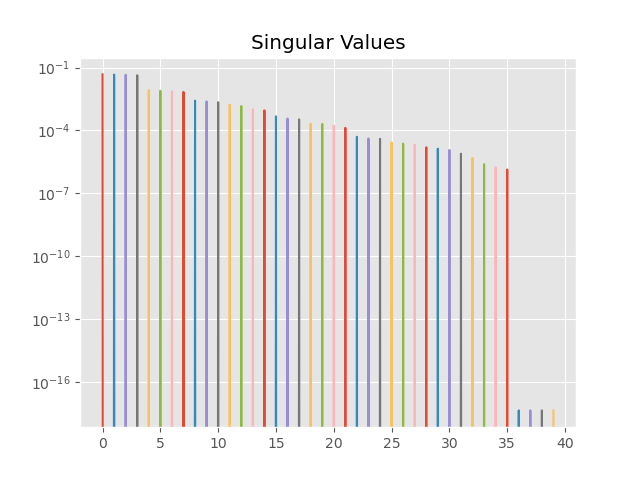
\includegraphics[width=\linewidth]{quest_svd-A_S_eVals.png}
      \caption{Singular Values}
      \label{fig:eVals}
    \end{figure}

    \begin{figure}
      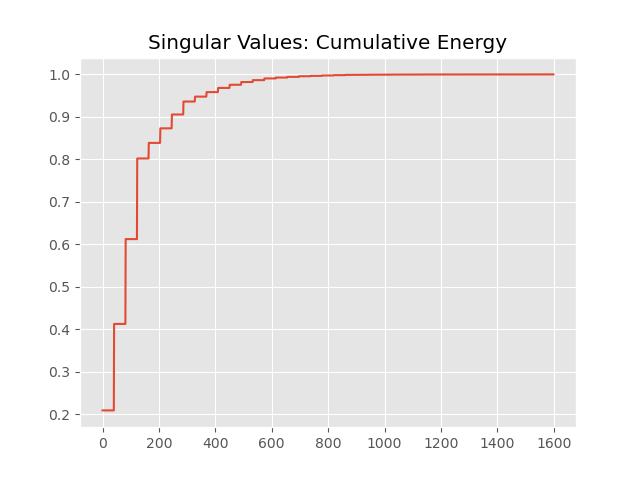
\includegraphics[width=\linewidth]{quest_svd-A_S_cumEnergy.png}
      \caption{Singular Value Cumulative Sum}
      \label{fig:cumsum}
    \end{figure}


    Back to discussing null space created in a situation where we aim to compute
    the coordinate transformation between two image frames. Given a set of
    matched correspondences, we aim to compute the closest linear transform
    between the two frames. Instead of using RANSAC which is too costly, we can
    simply compute the nearest orthogonal matrix. We know that the
    transformation is linear, the solution must be unique, and the axis must be
    orthogonal. Thus, this becomes an optimization problem where we seek to
    find the linear transform solution that yields the smallest Euclidean
    distance as it maps the initial coordinate frame to the latter. The Kabsch
    algorithm (also known as Wahba's problem) claims to provide an optimal
    method for computing the nearest orthogonal matrix
    \cite{kabsch1978discussion}. There is an
    implementation of this algorithm available in Scipy \cite{scipyspa85:online}.



    \item DLO Manipulation Milestones: I am hesitant to move forward the DLO
    project after VPQEKF project for multiple reasons. 1) It is too advanced of
    a problem and I may not be able to finish it the way I want by the end of my
    Ph.D. studies, 2) the market oppertunity is little for such technology and
    at this point it is of extreme strategic importance to me to achieve low cost
    mass production with priority with items with the largest margin. We can
    keep working on the proposal but I would not spend my own time and money on
    it at this point. 3) To achieve DLO manipulation, first I must achieve
    manipulation of rigid objects first and the best approach for that in my
    opinion is easily available dataset. I think it is strategically important to
    streamline the data acquisition and annotation process. So I have shared
    my ideas about making a 3D object scanner and I have some ideas for
    generating groundtruth automatically or with minimal input. For known objects,
    I will define grasping normals and surfaces that can be stored onboard. Thus,
    the grasping problem will be reduced to pose estimation of known objects.


    \item 3D Scanner: It is needed for object manipulation and perception tasks.
    \item Pose Estimation (\textcolor{blue}{DLO-01}): On-going under VPQEKF.
    \item Semantic segmentation (\textcolor{blue}{DLO-02}): Per my discussion with Dr. Gans, I
    will explore DL methods for the depth or scale problem.
    \item Grasping Project (\textcolor{blue}{DLO-03}): I am making this a part of the DLO project.
    \item PyTorch Tutorials: Transfer learning.

  \end{itemize}

\section{Intermediate Goals - Fall 2021:}
\begin{itemize}
      \item QEKF: Finish paper.
      \item UR5e: Do the tutorials.
\end{itemize}

\newpage

%Sets the bibliography style to UNSRT and import the
\newpage
\bibliography{ref}
\bibliographystyle{ieeetr}

\end{document}
